\chapter{Modèle SIR} \label{ch:intro}

\section{Mesures et méthodologie SIR}

Les mesures ainsi que les méthodologie sont les mêmes que pour le modèle SI, c'est-à-dire que les densité $\frac{1}{2},\frac{1}{4},\frac{1}{8},\frac{1}{16}$ et les tailles de populations $5000,20000,50000,100000$ sont étudiées.

\subsection{Résultats}

\begin{figure}[h]
	\centering
	\captionsetup{justification=centering}
	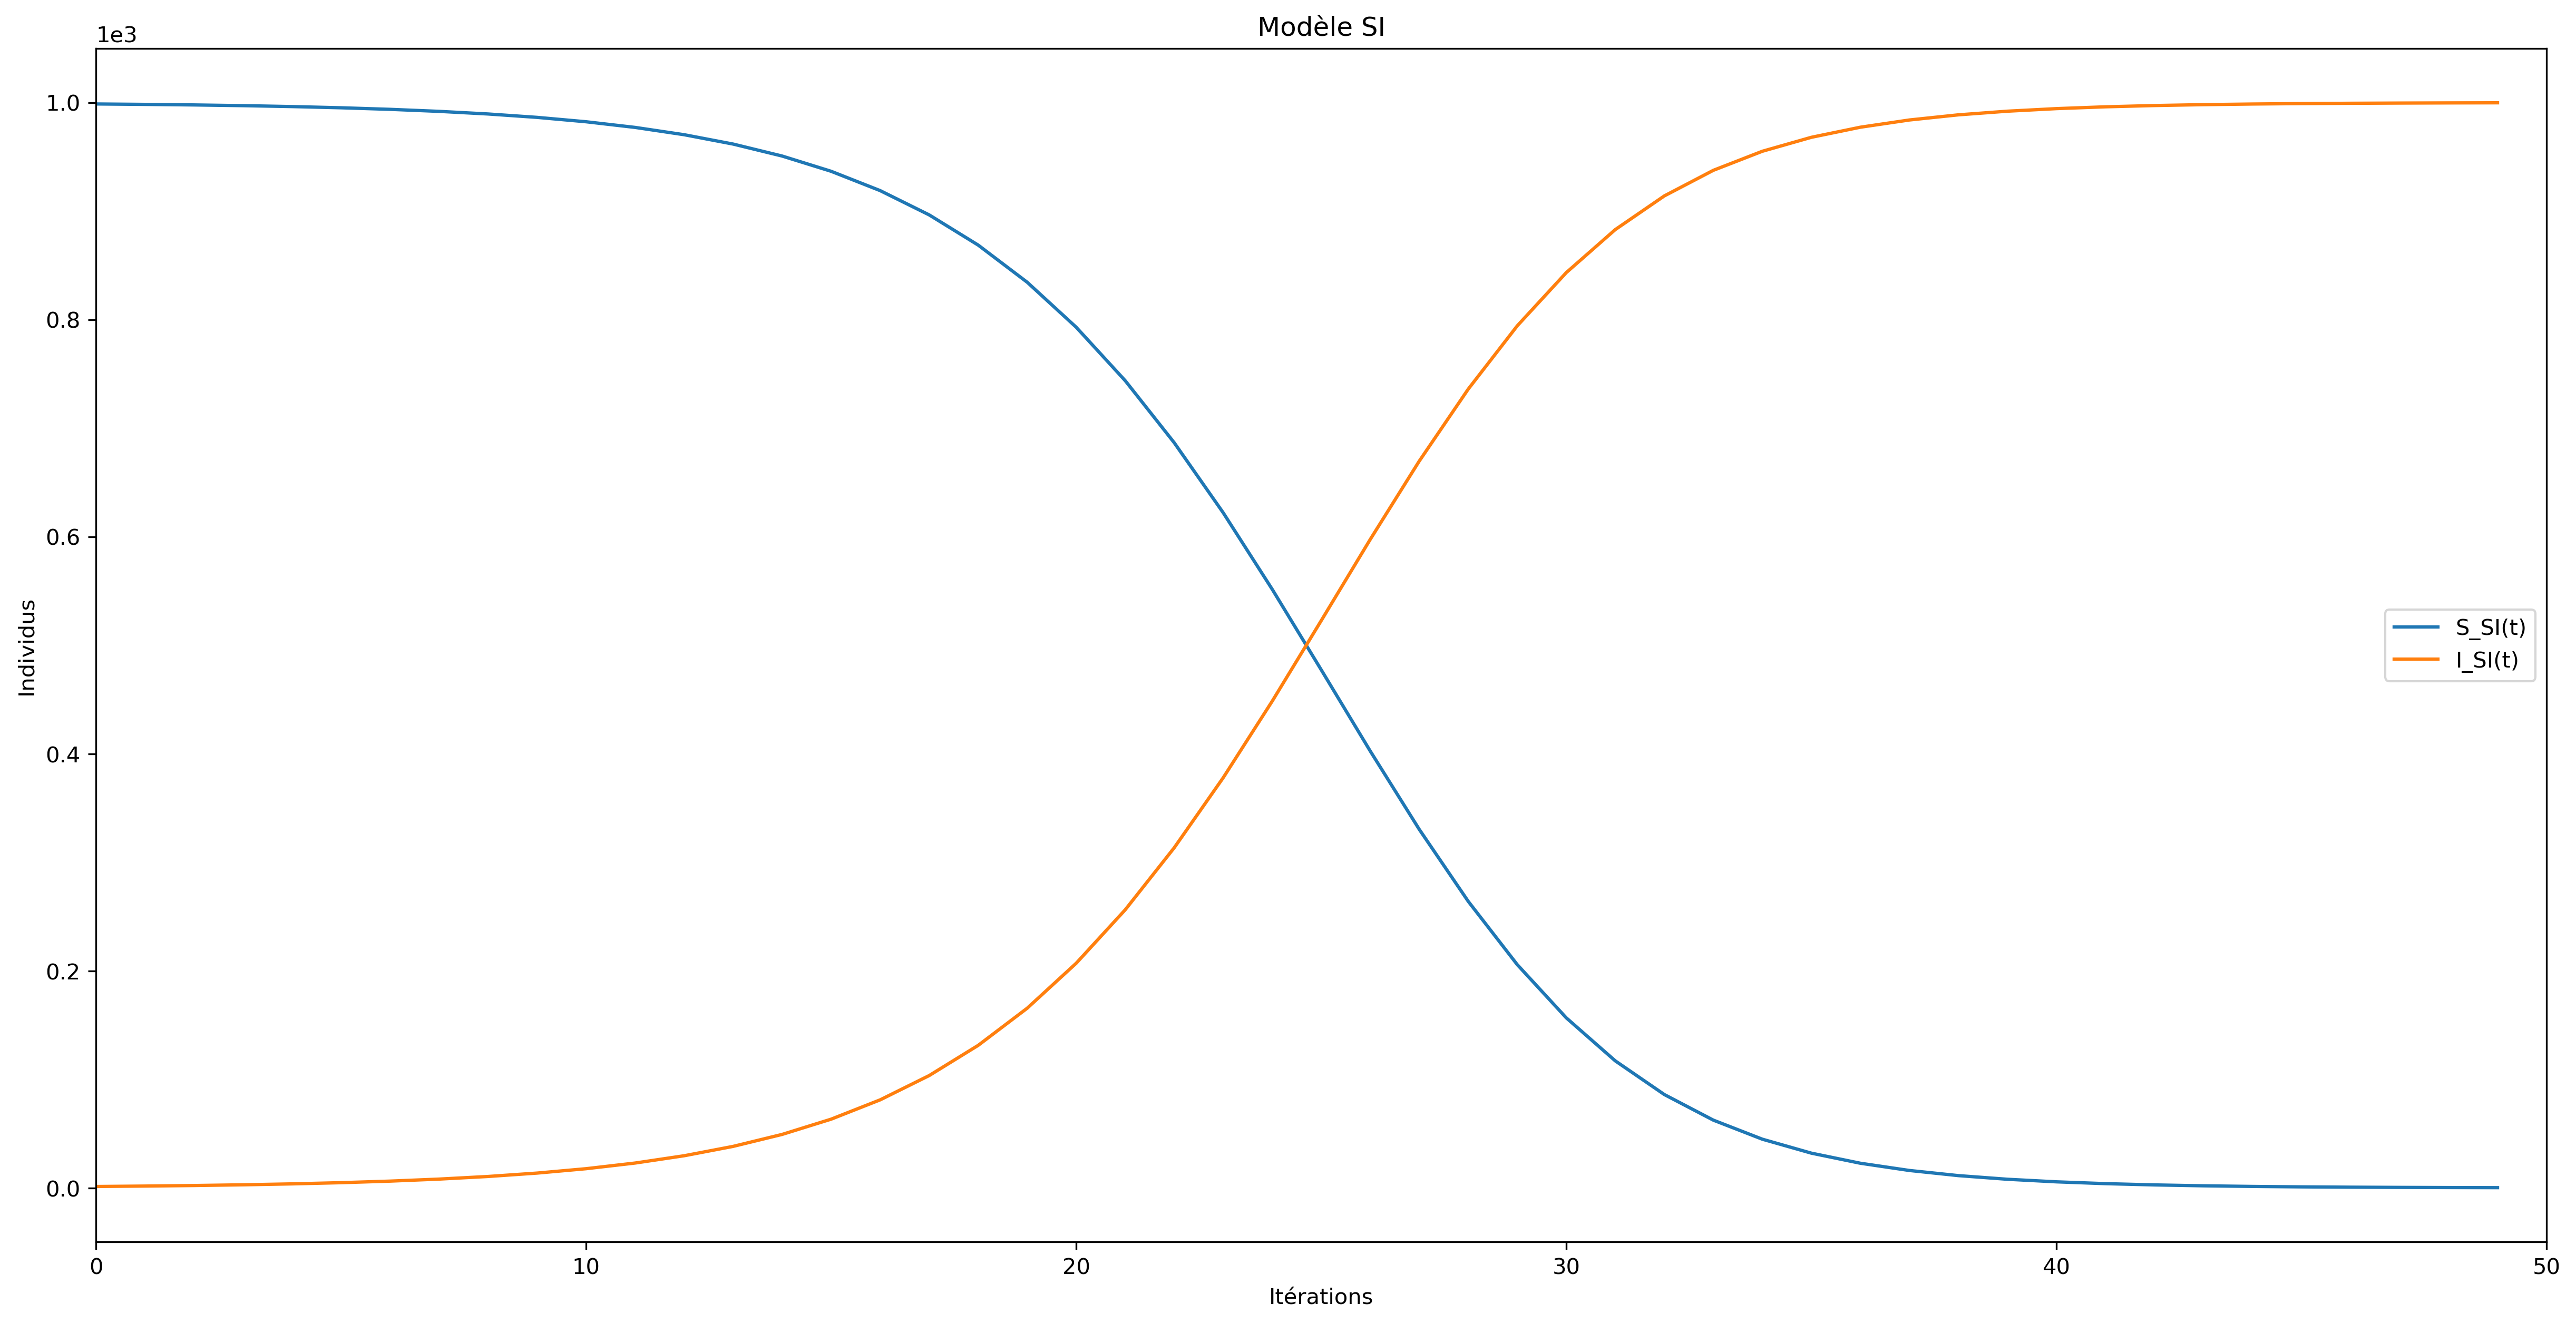
\includegraphics[width=.4\textwidth]{Images/SI_exemple.png}
	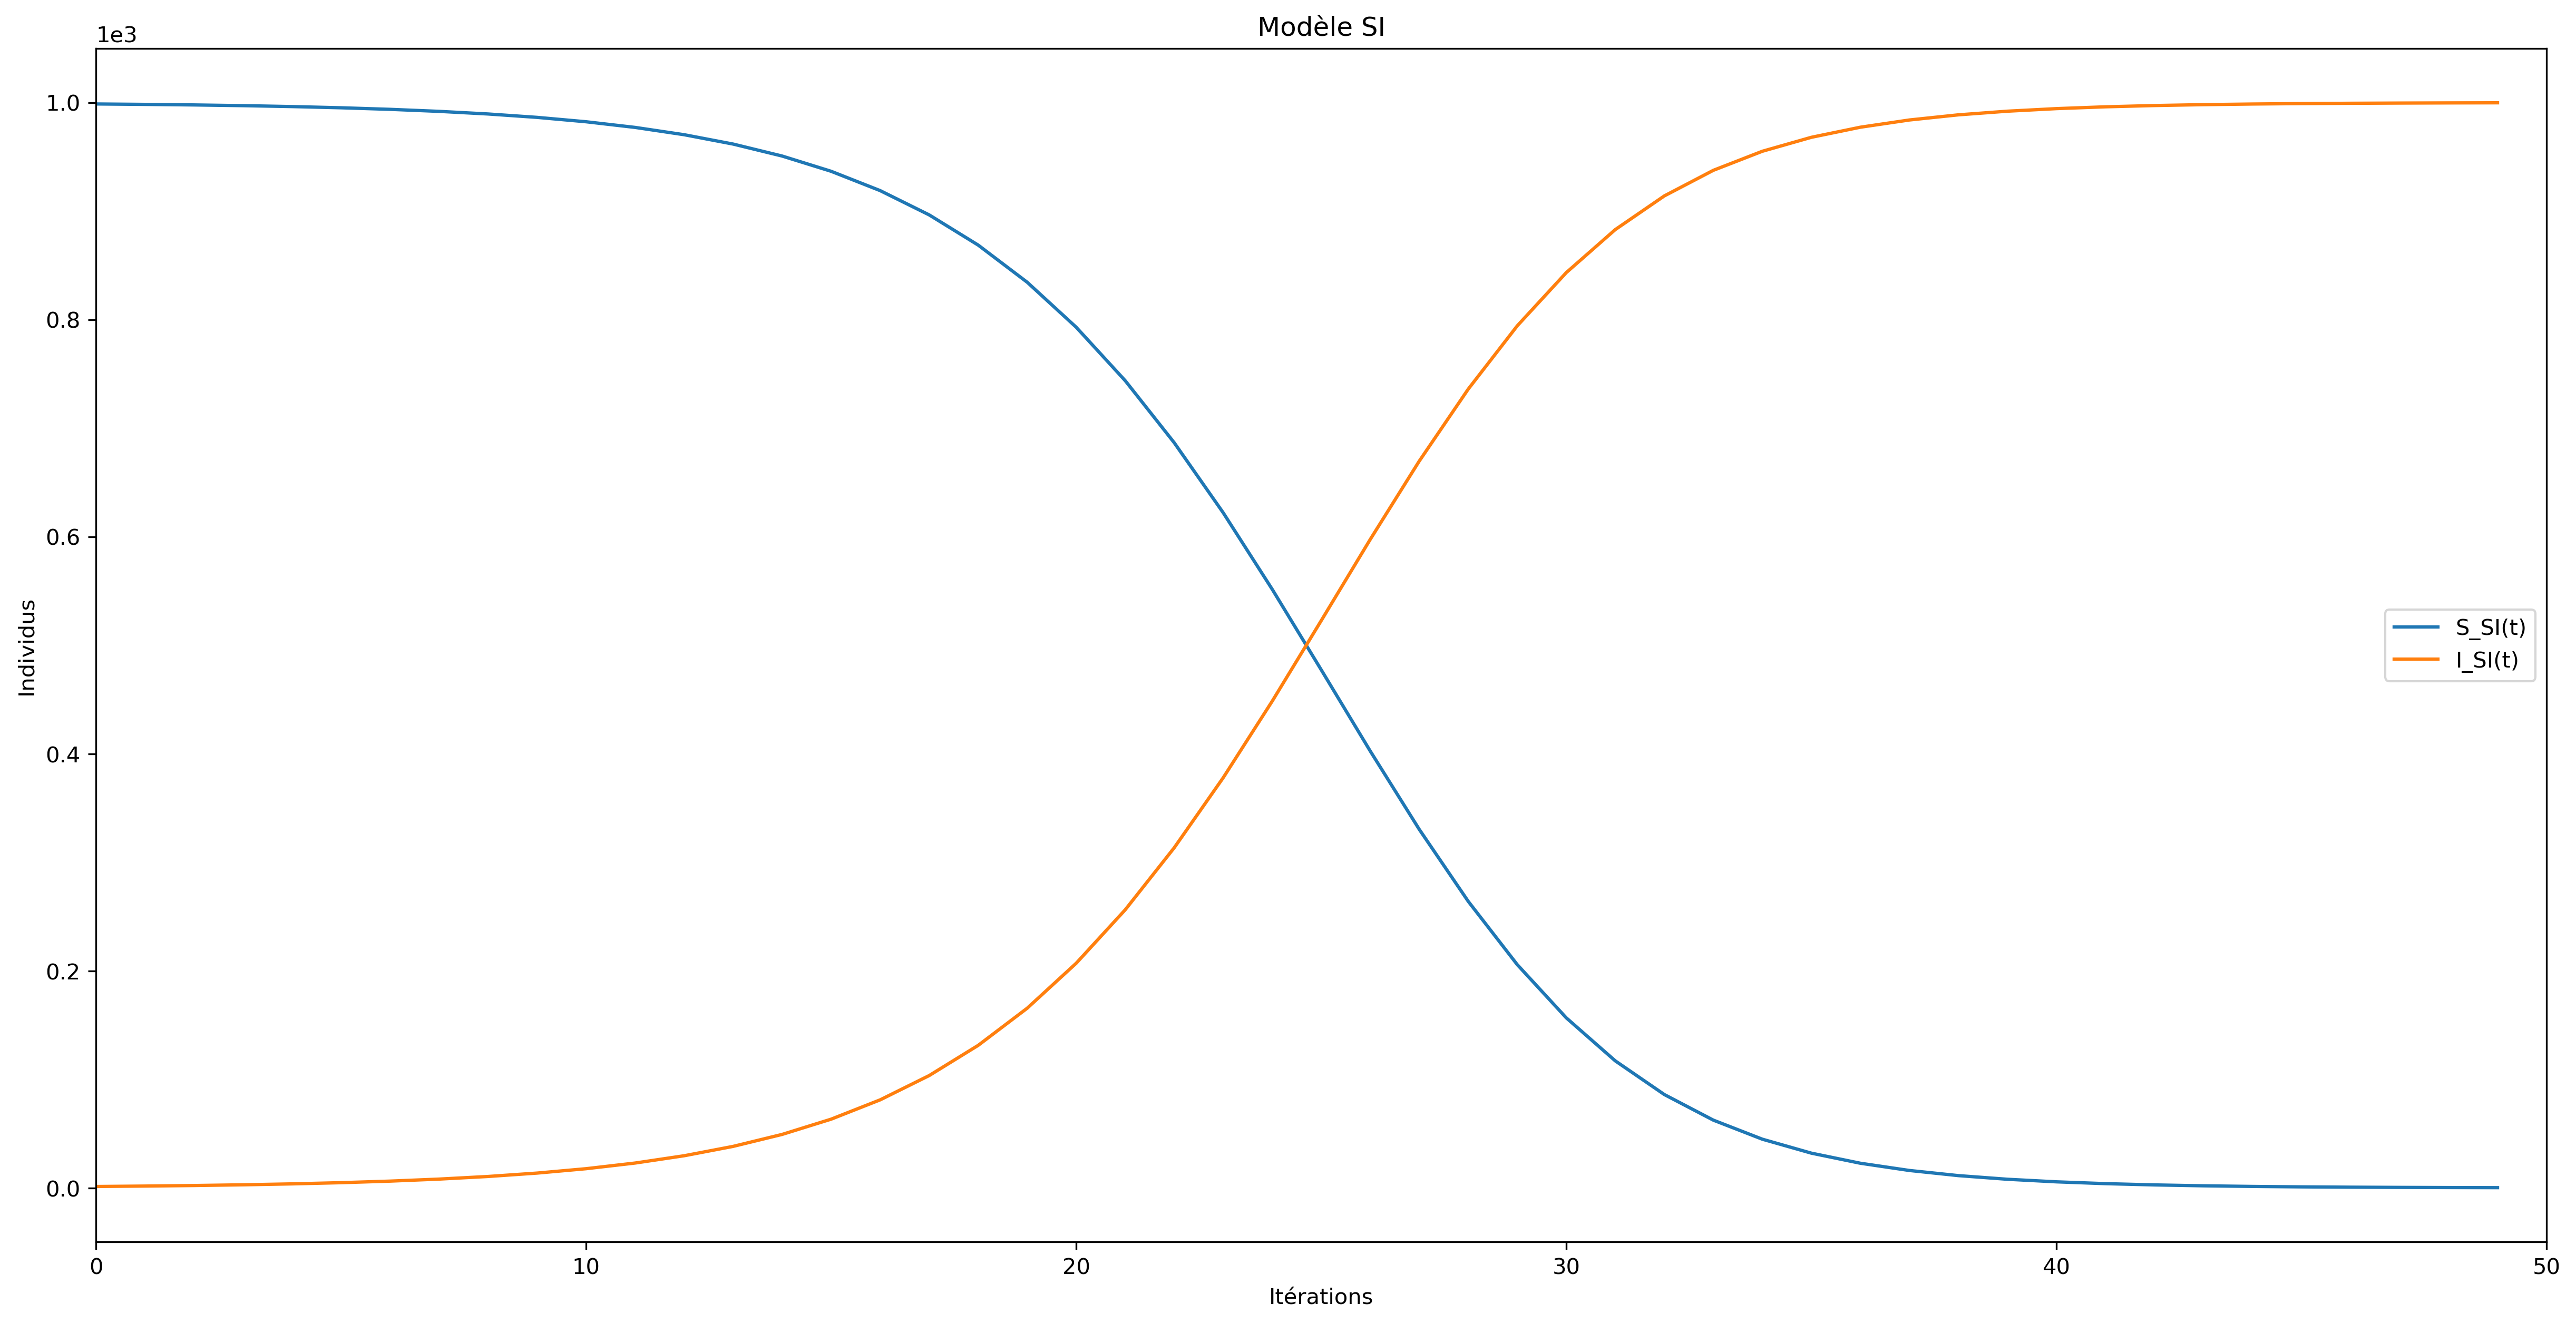
\includegraphics[width=.4\textwidth]{Images/SI_exemple.png}
	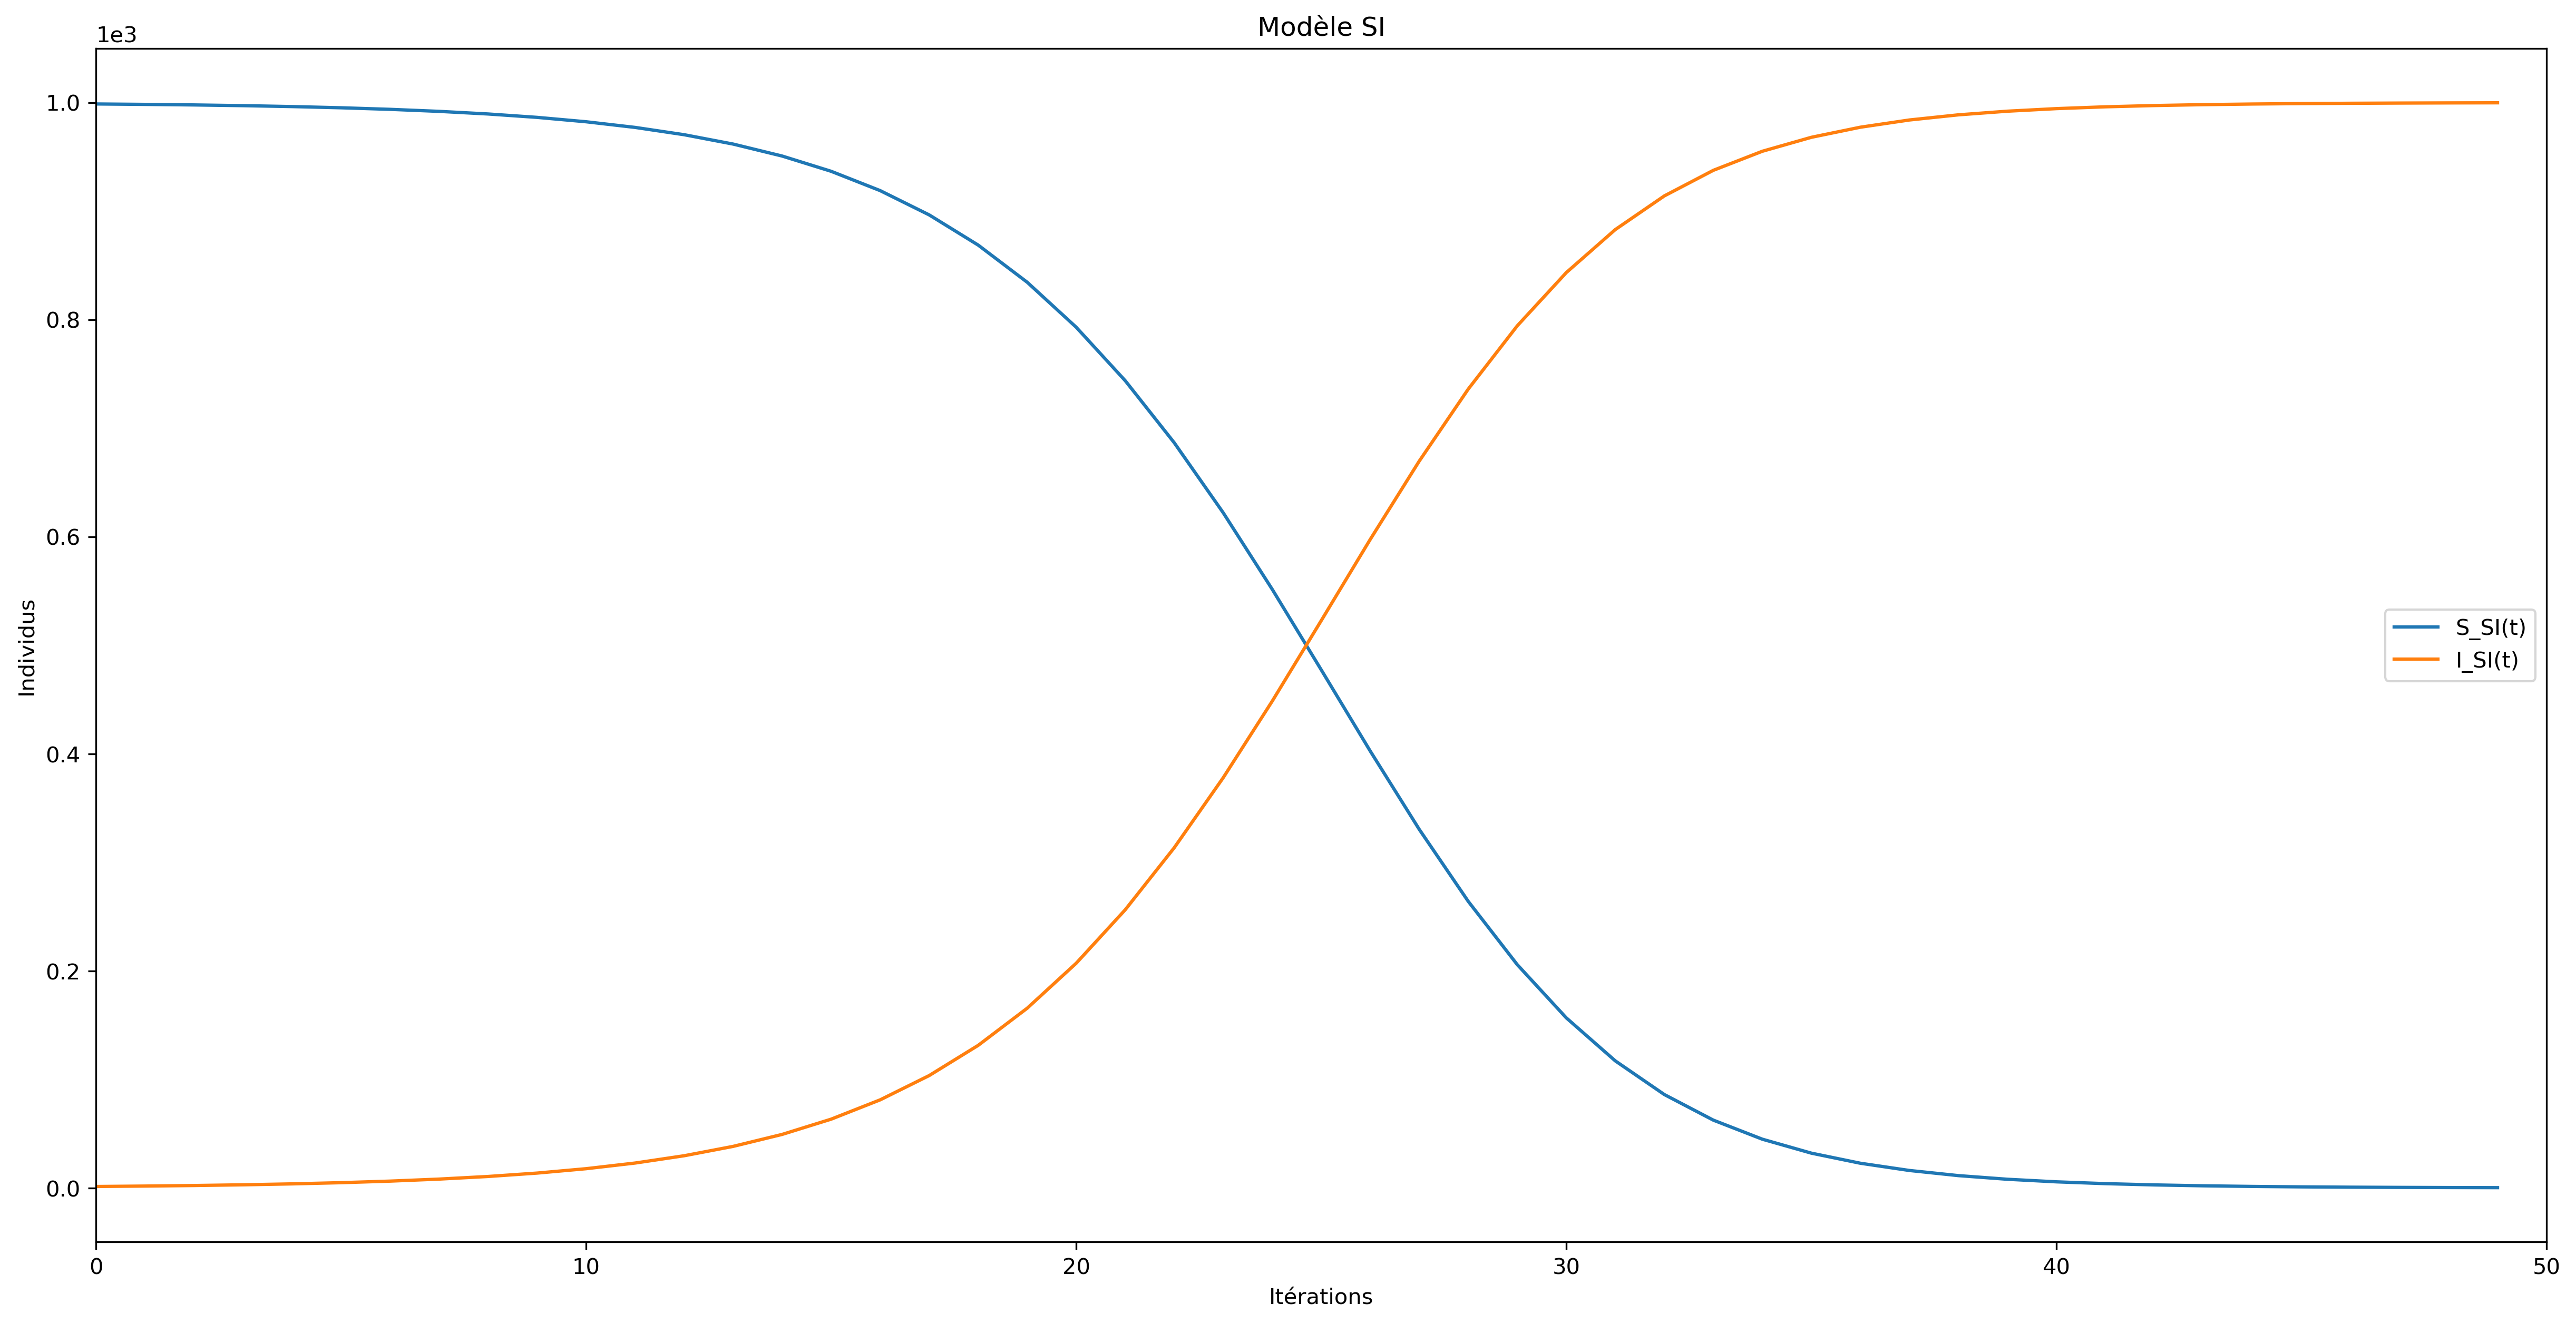
\includegraphics[width=.4\textwidth]{Images/SI_exemple.png}
	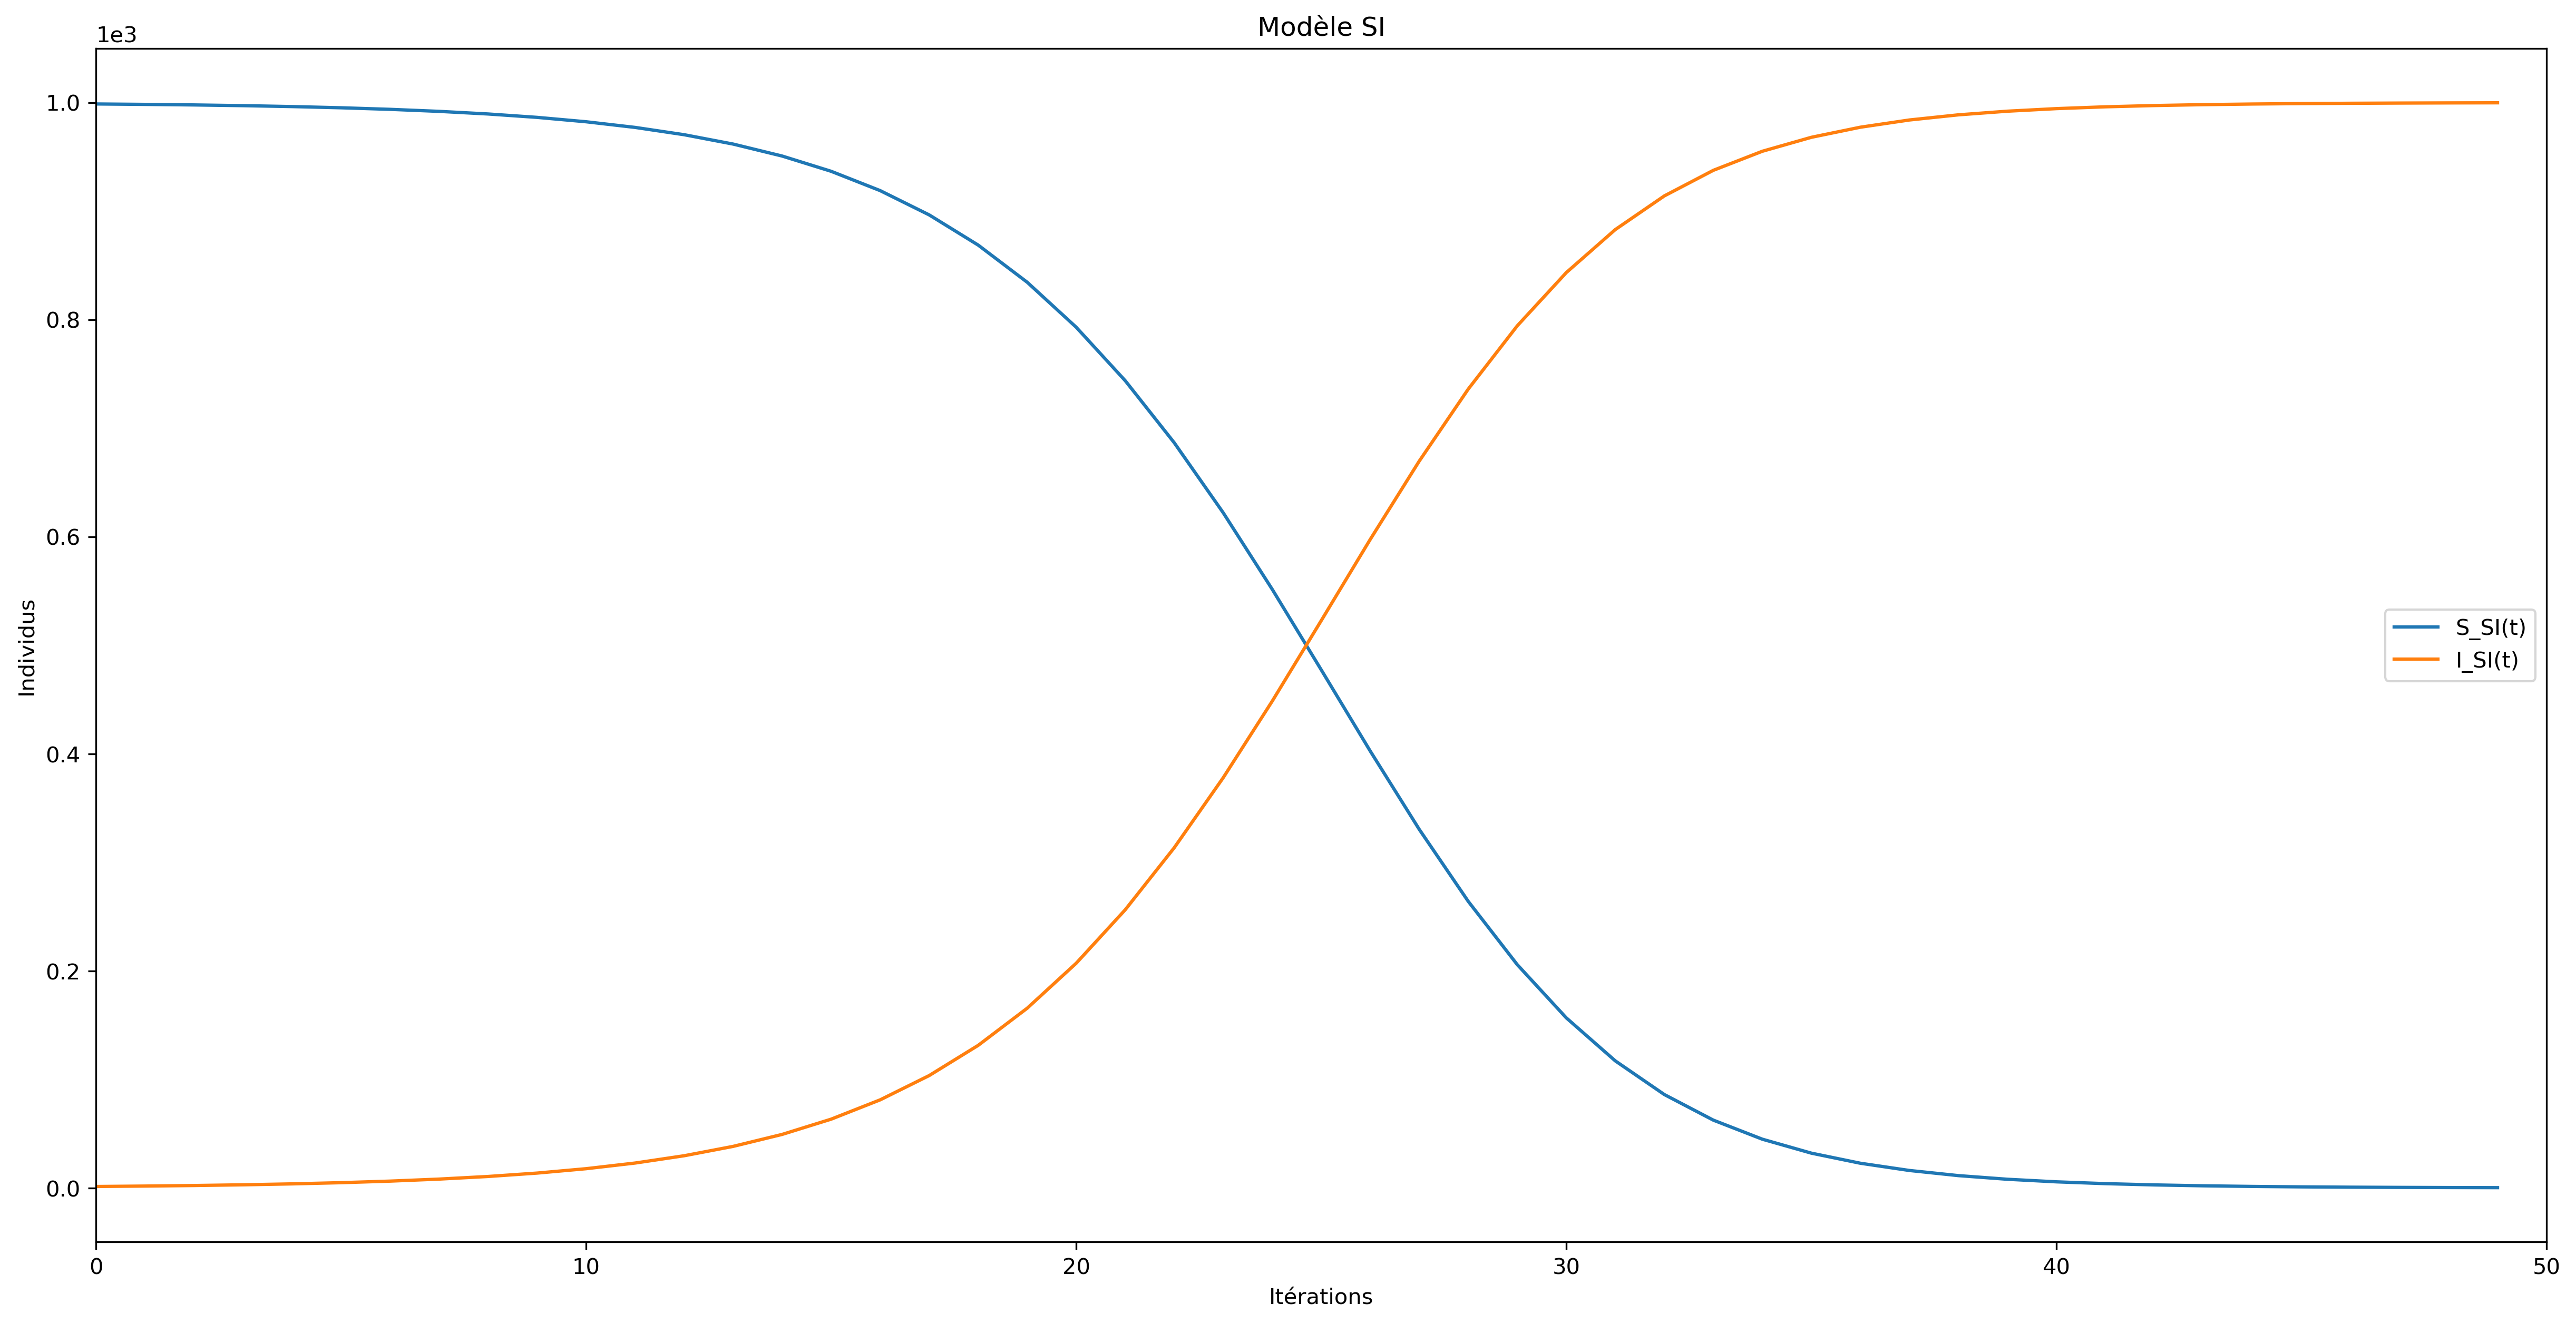
\includegraphics[width=.4\textwidth]{Images/SI_exemple.png}
	\caption{test}
\end{figure}
